% -*- coding: utf-8 -*-
% (begin (set! index 1) ((lambda ...) ... ))
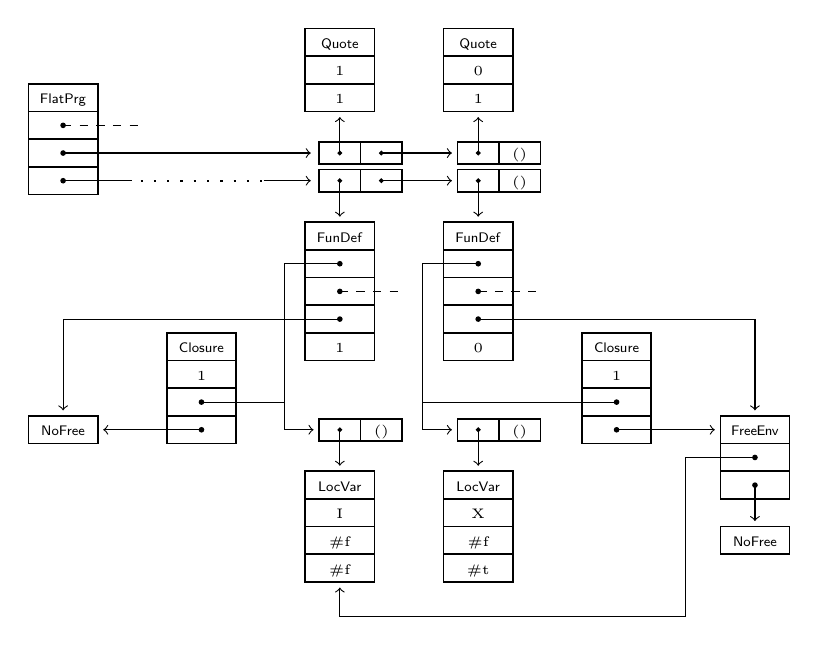
\begin{tikzpicture}
  \tikzstyle{every node}=[font=\tiny]

\def\NodeContent#1{\node [anchor = mid] at(1.25em, -0.5em) {#1};}
\def\NodeTitle#1{\NodeContent{\textsf{#1}}}
\def\NodePtr{\filldraw (1.25em, -0.5em) circle(0.8pt);}
\def\Box{\draw [semithick] (0, 0) rectangle (2.5em, -1.0em);}

\def\InList{%
  \begin{scope}[xshift = +0.5em, yshift = +1.5em]
    \draw [semithick] (0.0em, +0.4em) rectangle (3.0em, -0.4em)
                      (1.5em, +0.4em) -- (1.5em, -0.4em);
    \filldraw (0.75em, 0.0em) circle(0.65pt)
              (2.25em, 0.0em) circle(0.65pt);
  \end{scope}
}

\def\InListLast{%
  \begin{scope}[xshift = +0.5em, yshift = +1.5em]
    \draw [semithick] (0.0em, +0.4em) rectangle (3.0em, -0.4em)
                      (1.5em, +0.4em) -- (1.5em, -0.4em);
    \filldraw (0.75em, 0.0em) circle(0.65pt);
    \node [anchor = mid] at(2.25em, 0.0em) {\ic{()}};
  \end{scope}
}

\def\PullListLink{\draw [->] (-2.25em, 1.5em) -- (0.30em, 1.5em);}

\def\InBotList{%
  \begin{scope}[xshift = +0.5em, yshift = -1.5em]
    \draw [semithick] (0.0em, +0.4em) rectangle (3.0em, -0.4em)
                      (1.5em, +0.4em) -- (1.5em, -0.4em);
    \filldraw (0.75em, 0.0em) circle(0.65pt)
              (2.25em, 0.0em) circle(0.65pt);
  \end{scope}
}

\def\InBotListLast{%
  \begin{scope}[xshift = +0.5em, yshift = -1.5em]
    \draw [semithick] (0.0em, +0.4em) rectangle (3.0em, -0.4em)
                      (1.5em, +0.4em) -- (1.5em, -0.4em);
    \filldraw (0.75em, 0.0em) circle(0.65pt);
    \node [anchor = mid] at(2.25em, 0.0em) {\ic{()}};
  \end{scope}
}

\def\PullBotListLink{\draw [->] (-2.25em, -1.5em) -- (0.30em, -1.5em);}

\def\PullLinkUp{\draw    [->] ( 1.25em,  1.50em) -- ( 1.25em,  0.20em);}
\def\PullLinkLeft{\draw  [->] (-3.75em, -0.50em) -- (-0.20em, -0.50em);}
\def\PullLinkDown{\draw  [->] ( 1.25em, -1.50em) -- ( 1.25em, -0.20em);}
\def\PullLinkRight{\draw [->] ( 6.25em, -0.50em) -- ( 2.70em, -0.50em);}

\def\NoArgNode{%
  \begin{scope}[yshift = -0.0em]
    \Box
    \NodeTitle{NoArg}
  \end{scope}
}

\def\NoFreeNode{%
  \begin{scope}[yshift = -0.0em]
    \Box
    \NodeTitle{NoFree}
  \end{scope}
}

\def\PtrNodeU#1{%
  \begin{scope}[yshift = -0.0em]
    \Box
    \NodeTitle{#1}
  \end{scope}
  \begin{scope}[yshift = -1.0em]
    \Box
    \NodePtr
  \end{scope}
}

\def\ContentNode#1#2{
  \begin{scope}[yshift = -0.0em]
    \Box
    \NodeTitle{#1}
  \end{scope}
  \begin{scope}[yshift = -1.0em]
    \Box
    \NodeContent{#2}
  \end{scope}
}

\def\PtrNodeD#1{%
  \begin{scope}[yshift = -0.0em]
    \Box
    \NodeTitle{#1}
  \end{scope}
  \begin{scope}[yshift = -1.0em]
    \Box
    \NodePtr
  \end{scope}
  \begin{scope}[yshift = -2.0em]
    \Box
    \NodePtr
  \end{scope}
}

\def\ContentNodeD#1#2#3{
  \begin{scope}[yshift = -0.0em]
    \Box
    \NodeTitle{#1}
  \end{scope}
  \begin{scope}[yshift = -1.0em]
    \Box
    \NodeContent{#2}
  \end{scope}
  \begin{scope}[yshift = -2.0em]
    \Box
    \NodeContent{#3}
  \end{scope}
}

\def\PtrNodeDS#1{%
  \begin{scope}[yshift = -0.0em]
    \Box
    \NodeTitle{#1}
  \end{scope}
  \begin{scope}[yshift = -1.0em]
    \Box
    \begin{scope}[xshift = +0.35em]
      \NodePtr
    \end{scope}
  \end{scope}
  \begin{scope}[yshift = -2.0em]
    \Box
    \begin{scope}[xshift = -0.35em]
      \NodePtr
    \end{scope}
  \end{scope}
}

\def\PtrNodeT#1{
  \begin{scope}[yshift = -0.0em]
    \Box
    \NodeTitle{#1}
  \end{scope}
  \begin{scope}[yshift = -1.0em]
    \Box
    \NodePtr
  \end{scope}
  \begin{scope}[yshift = -2.0em]
    \Box
    \NodePtr
  \end{scope}
  \begin{scope}[yshift = -3.0em]
    \Box
    \NodePtr
  \end{scope}
}

\def\LocVarNode#1#2#3{
  \begin{scope}[yshift = -0.0em]
    \Box
    \NodeTitle{LocVar}
  \end{scope}
  \begin{scope}[yshift = -1.0em]
    \Box
    \NodeContent{#1}
  \end{scope}
  \begin{scope}[yshift = -2.0em]
    \Box
    \NodeContent{#2}
  \end{scope}
  \begin{scope}[yshift = -3.0em]
    \Box
    \NodeContent{#3}
  \end{scope}
}

\def\ClosureNode#1{
  \begin{scope}[yshift = -0.0em]
    \Box
    \NodeTitle{Closure}
  \end{scope}
  \begin{scope}[yshift = -1.0em]
    \Box
    \NodeContent{#1}
  \end{scope}
  \begin{scope}[yshift = -2.0em]
    \Box
    \NodePtr
  \end{scope}
  \begin{scope}[yshift = -3.0em]
    \Box
    \NodePtr
  \end{scope}
}

\def\FunDefNode#1{
  \begin{scope}[yshift = -0.0em]
    \Box
    \NodeTitle{FunDef}
  \end{scope}
  \begin{scope}[yshift = -1.0em]
    \Box
    \NodePtr
  \end{scope}
  \begin{scope}[yshift = -2.0em]
    \Box
    \NodePtr
  \end{scope}
  \begin{scope}[yshift = -3.0em]
    \Box
    \NodePtr
  \end{scope}
  \begin{scope}[yshift = -4.0em]
    \Box
    \NodeContent{#1}
  \end{scope}
}


\begin{scope}[xshift = 0.0em]
    \begin{scope}[yshift =  -0.0em]
        \PtrNodeT{FlatPrg}
    \begin{scope}[yshift = -12.0em]
        \NoFreeNode
        \PullLinkRight
    \end{scope}\end{scope}
\end{scope}

% FlagPrg ->
\draw [dashed] (1.25em, -1.50em) -- ( 4.00em, -1.50em);

% FlagPrg -> (Quote)
\draw [->]     (1.25em, -2.50em) -- (10.20em, -2.50em);

% FlagPrg -> (FunDef)
\draw                         (1.25em, -3.50em) -- ( 3.75em, -3.50em);
\draw [loosely dotted, thick] (4.05em, -3.50em) -- ( 8.45em, -3.50em);
\draw [->]                    (8.50em, -3.50em) -- (10.20em, -3.50em);

\begin{scope}[xshift = 5.0em]
    \begin{scope}[yshift = -9.0em]
        \ClosureNode{\ic{1}}
    \end{scope}
\end{scope}

\begin{scope}[xshift = 10.0em]
    \begin{scope}[yshift = +2.0em]
        \ContentNodeD{Quote}{\ic{1}}{\ic{1}}
        \begin{scope}[yshift = -3.0em]
            \InBotList
            \PullLinkDown
        \end{scope}
    \end{scope}
    \begin{scope}[yshift = -5.0em]
        \InList
        \PullLinkUp
        \FunDefNode{\ic{1}}
    \begin{scope}[yshift = -9.0em]
        \InListLast
        \PullLinkUp
        \LocVarNode{\ic{I}}{\ic{\#f}}{\ic{\#f}}
    \end{scope}\end{scope}
\end{scope}

% FunDef -> (LocVar : I)
% Closure -> (LocVar : I)
\draw [->] (11.25em,  -6.50em) -- ( 9.25em,  -6.50em) --
           ( 9.25em, -12.50em) -- (10.30em, -12.50em);
\draw      ( 6.25em, -11.50em) -- ( 9.25em, -11.50em);

% FunDef ->
\draw [dashed] (11.25em, -7.50em) -- (13.50em, -7.50em);

% FunDef -> NoFree
\draw [->] (11.25em, -8.50em) -- (1.25em, -8.50em) -- (1.25em, -11.80em);

\begin{scope}[xshift = 15.0em]
    \begin{scope}[yshift = +2.0em]
        \ContentNodeD{Quote}{\ic{0}}{\ic{1}}
        \begin{scope}[yshift = -3.0em]
            \InBotListLast
            \PullLinkDown
            \PullBotListLink
        \end{scope}
    \end{scope}
    \begin{scope}[yshift = -5.0em]
        \InListLast
        \PullLinkUp
        \PullListLink
        \FunDefNode{\ic{0}}
    \begin{scope}[yshift = -9.0em]
        \InListLast
        \PullLinkUp
        \LocVarNode{\ic{X}}{\ic{\#f}}{\ic{\#t}}
    \end{scope}\end{scope}
\end{scope}

% FunDef -> (LocVar : X)
% Closure -> (LocVar : X)
\draw [->] (16.25em,  -6.50em) -- (14.25em,  -6.50em) --
           (14.25em, -12.50em) -- (15.30em, -12.50em);
\draw      (21.25em, -11.50em) -- (14.25em, -11.50em);

% FunDef ->
\draw [dashed] (16.25em, -7.50em) -- (18.50em, -7.50em);

% FunDef -> FreeEnv
\draw [->] (16.25em, -8.50em) -- (26.25em, -8.50em) -- (26.25em, -11.80em);

\begin{scope}[xshift = 20.0em]
    \begin{scope}[yshift = -9.0em]
        \ClosureNode{\ic{1}}
    \end{scope}
\end{scope}

\begin{scope}[xshift = 25.0em]
    \begin{scope}[yshift = -12.0em]
        \PullLinkLeft
        \PtrNodeD{Free{\kern-0.03em}E{\kern-0.04em}n{\kern-0.05em}v}
    \begin{scope}[yshift =  -4.0em]
        \PullLinkUp
        \NoFreeNode
    \end{scope}\end{scope}
\end{scope}

% FreeEnv -> LocVar : I
\draw [->] (26.25em, -13.50em) -- (23.75em, -13.50em) -- (23.75em, -19.25em) --
           (11.25em, -19.25em) -- (11.25em, -18.20em);

\end{tikzpicture}
